\chapter{Generating Markov Chains With the PECOS Toolkit}\label{ch-gmc}
\thispagestyle{headings}
\markboth{Chapter \ref{ch-gmc}: Generating Markov Chains with the PECOS Toolkit}{Chapter \ref{ch-gmc}: Generating Markov Chains With the PECOS Toolkit}

The PECOS Toolkit currently implements the DRAM algorithm \cite{HaLaMiSa06} for the generation of a Markov chain.
Section \ref{sc-gmc-seven-steps} explains how to develop your own application using the DRAM capabilities of the PECOS Toolkit, while
Section \ref{sc-gmc-dram-output} describes the output information generated by the toolkit and
Sections
\ref{sc-gmc-dram-normal-ex},
\ref{sc-gmc-dram-chem-ex} and
\ref{sc-gmc-dram-algae-ex}
describe the three examples available,
all of them also available in \cite{mcmctool}.

The chapter ends at Section \ref{sc-gmc-planned-features} with a brief list of planned features for next toolkit versions w.r.t. Markov Chain Monte Carlo methods.

\section{Seven Steps}\label{sc-gmc-seven-steps}

The process of developing an application (let us call it ``newexample'') 
that uses the DRAM implementation of the PECOS Toolkit involves the following seven steps:
\begin{enumerate}
\item prepare a file describing the {\it system input parameters}; let us call it ``newexample.par''; see Subsection \ref{subsc-gmc-seven-steps-sys-input-params};
\item create your {\it code directory}; let us call it ``uq/appls/mcmc/newexample''; See Subsection \ref{subsc-gmc-seven-steps-myexample};
\item if necessary, compute your {\it proposal covariance matrix} for the $q_1(\cdot,\cdot)$ proposal transition probability kernel; the PECOS library will internally compute a default covariance matrix if the user does not supply one; see Subsection \ref{subsc-gmc-seven-steps-proposal-cov-matrix-for-q1};
\item if necessary, code your {\it prior function}; there is a default prior in the PECOS library; see Subsection \ref{subsc-gmc-seven-steps-prior-code};
\item code your {\it likelihood function}, which returns a vector of values, each value corresponding to the likelihood of a specific output quantity, as explained in Section \ref{sc-intro-qoi}, page \pageref{sc-intro-qoi}; see Subsection \ref{subsc-gmc-seven-steps-likelihood-code};
\item {\it compile} your code; see Subsection \ref{subsc-gmc-seven-steps-compile};
\item prepare an input file setting the {\it algorithm parameters}; let us call it ``newexample.inp''; see Subsection \ref{subsc-gmc-seven-steps-alg-params}.
\end{enumerate}
Finally, {\it run} your application by executing ``./newexample -i newexample.inp''.

\subsection{File Describing System Input Parameters}\label{subsc-gmc-seven-steps-sys-input-params}

{\it All system input parameters are assumed to be scalar r.v.'s} (that is, $n_i=1,~i=1,2,\ldots,n_{\text{sip}}$, according to the terminology of Section \ref{sc-intro-qoi}), and
have to be specified in a file.
This file describing system input parameters contains a lot of prior information as well.
It is treated by the PECOS Toolkit as having either parameter lines or comment lines.
Comment lines are all those that begin with the character ``\#'', otherwise they are treated as parameter lines.
Comment lines can appear anywhere in the line.
Each parameter line is related to one input parameter.
The first parameter line specifies the input parameter $\theta_0$,
the second parameter line specifies the input parameter $\theta_1$,
and so on.
Let us ``$i$'' denote the index for the input parameter $\theta_i$.
From left to right, each parameter line shall contain the following fields separated by black space(s):
\begin{itemize}
\item name of $\theta_i$, without spaces: this field is mandatory;
\item $\theta_i^{(0)}$, the component value on the initial sample of the chain: this field is also mandatory;
\item $\theta_{i,\text{min}}$, the minimum value allowed for this component during chain generation, otherwise the candidate position is rejected: this field is optional and its default value is ``-inf'';
\item $\theta_{i,\text{max}}$, the maximum value allowed for this component during chain generation, otherwise the candidate position is rejected: this field is optional and its default value is ``inf'';
\item $E_{\text{prior}}[\theta_i]$, the expected value of the input parameter; this field is optional and the default value is ``nan'';
\item $V_{\text{prior}}[\theta_i]$, the variance of the input parameter; this field is optional and the default value is ``inf''.
\end{itemize}
If a parameter line is improperly set, the code will exit with a failure message.
An example of an input file is shown in Figure \ref{fig-dram-par-file-ex}.

\begin{figure}[h!]
\begin{verbatim}
# This is the file of system input parameters for "newexample".
# Tha name of this file must match the entry "uqParamSpace_inputFile" in
# the input file.
# Lines that begin with the character `#' are considered comment lines.
# Each line that is not a comment line is treated as representing an input
# parameter.
# From left to right, the entries in each input parameter line correspond to:
# --> parameter name (mandatory)
# --> initial value (mandatory)
# --> minimum value (optional; default value to "-inf")
# --> maximum value (optional; default value to "inf")
# --> expectation (optional; default value to "nan")
# --> variance (optional; default value to "inf")
Name_1 0. -inf
# Comment lines can appear anywhere in the file.
Name_2 0. -inf inf 0. inf
Name_3 0.
Name_4 0. -inf inf 0. inf
# The total number of input parameter lines (4 in this example) must match
# the entry "uqParamSpace_dim" in the input file.
\end{verbatim}
\caption{Example of the specification of system input parameters for the generation of a Markov chain by the PECOS Toolkit.
}
\label{fig-dram-par-file-ex}
\end{figure}

\subsection{Creating Your Code Directory}\label{subsc-gmc-seven-steps-myexample}

\begin{itemize}
\item execute ``uq/appls/mcmc/newexample'';
\item execute ``cp -R template newexample'';
\item execute ``cd newexample'';
\item change ``template'' and ``Template'' to ``newexample'' and ``newexample'' in all files, including the file ``Makefile''.
\end{itemize}

\subsection{The Proposal Covariance Matrix for $q_1(\cdot,\cdot)$}\label{subsc-gmc-seven-steps-proposal-cov-matrix-for-q1}
$~$\\

\subsection{Code for the Prior Function}\label{subsc-gmc-seven-steps-prior-code}

The user might need to specify a prior probability density $\pi_{\text{prior}}(\boldsymbol{\theta})$
by passing to the PECOS Toolkit the address of a routine $f_{\text{user}}(\boldsymbol{\theta})$ that computes
\begin{equation}\label{eq-m2l-prior}
f_{\text{user}}(\boldsymbol{\theta})=
-2~ln~
\left[
\pi_{\text{prior}}(\boldsymbol{\theta})
\right].
\end{equation}
The code then computes
\begin{equation*}
\pi_{\text{prior}}(\boldsymbol{\theta}) = e^
{
\left\{
-\frac{1}{2}
f_{\text{user}}(\boldsymbol{\theta})
\right\}
}.
\end{equation*}

But the user specficication of a prior density is not mandatory, since the toolkit provides a default prior density given by
\begin{equation*}
\pi_{\text{prior,default}}(\boldsymbol{\theta}) =
e^{
\left\{
-\frac{1}{2}
(\boldsymbol{\theta}-E_{\text{prior}}[\boldsymbol{\theta}])^T
~C_{\text{prior}}^{-1}~
(\boldsymbol{\theta}-E_{\text{prior}}[\boldsymbol{\theta}])
\right\}
},
\end{equation*}
where the default covariance matrix $C_{\text{prior}}$ is the $n_{\text{sip}}\times n_{\text{sip}}$ diagonal matrix given by
\begin{equation}\label{eq-default-prior-cov-matrix}
C_{\text{prior}} =
\left[
\begin{array}{cccccc}
V_{\text{prior}}[\theta_1] & 0                          & 0                          & \ldots & 0                                           & 0      \\
0                          & V_{\text{prior}}[\theta_2] & 0                          & \ldots & 0                                           & 0      \\
0                          & 0                          & V_{\text{prior}}[\theta_3] & \ldots & 0                                           & 0      \\
\vdots                     & \vdots                     & \vdots                     & \ddots & \vdots                                      & \vdots \\
0                          & 0                          & 0                          & \ldots & V_{\text{prior}}[\theta_{n_{\text{sip}}-1}] & 0      \\
0                          & 0                          & 0                          & \ldots & 0                                           & V_{\text{prior}}[\theta_{n_{\text{sip}}}] \\
\end{array}
\right].
\end{equation}
In fact, in the spirit of \eqref{eq-m2l-prior}, the PECOS default prior routine computes
\begin{equation*}
(\boldsymbol{\theta}-E_{\text{prior}}[\boldsymbol{\theta}])^T
~C_{\text{prior}}^{-1}~
(\boldsymbol{\theta}-E_{\text{prior}}[\boldsymbol{\theta}]).
\end{equation*}
It should be noted that the values of $E_{\text{prior}}[\theta_i]$ and $V_{\text{prior}}[\theta_i]$, $i=1,2,\ldots,n_{\text{sip}}$,
are passed in the file of system input parameters described in Subsection \ref{subsc-gmc-seven-steps-sys-input-params}.

\subsection{Code for the Likelihood Function(s)}\label{subsc-gmc-seven-steps-likelihood-code}

The user must specify all likelihood densities $\ell_j(\mathbf{y}_{j,\text{obs}}|\boldsymbol{\theta})$, $j=1,2,\ldots,n_{\text{soq}}$,
by passing to the PECOS Toolkit the address of a routine that computes a vector $\mathbf{L}=(L_1,L_2,\ldots,L_{n_{\text{soq}}})\in\mathbb{R}^{N_{\text{soq}}}$  given by
\begin{equation}\label{eq-m2l-likelihood}
L_j = -2~V[\ell_j(\cdot)]~ln~
\left[
\ell_j(\mathbf{y}_{j,\text{obs}}|\boldsymbol{\theta})
\right],
\end{equation}
where
$V[\ell_j(\cdot)]$ denotes the model error variance, to be explained shortly.
The PECOS algorithm then computes
\begin{equation*}
\ell(\mathbf{y}_{\text{obs}}|\boldsymbol{\theta}) = e^
{
\left\{
-\frac{1}{2}\sum_{j=1}^{n_{\text{soq}}}~\frac{L_j}{V[\ell_j(\cdot)]}
\right\}
}.
\end{equation*}

Although these formulas seem strange, they are motivated by the fact that a common likelihood function is given by
\begin{equation*}
\ell_{\text{common}}(\mathbf{y}_{\text{obs}}|\boldsymbol{\theta}) =
\prod_{j=1}^{N_{\text{soq}}}~
e^
{
\left\{
-\frac{1}{2}~[m_j(\boldsymbol{\theta})-\mathbf{y}_{j,\text{obs}}]^T~\frac{1}{V[\ell_j(\cdot)]}~[m_j(\boldsymbol{\theta})-\mathbf{y}_{j,\text{obs}}]
\right\}
},
\end{equation*}
where
$m_j(\cdot)$ is the model function presented in \eqref{eq-m-j}, page \pageref{eq-m-j}.
In this case, the quantity $L_j$ becomes
\begin{equation}\label{eq-m2l-likelihood-2}
L_j = \|m_j(\boldsymbol{\theta})-\mathbf{y}_{j,\text{obs}}\|_2^2.
\end{equation}

\subsection{Compiling Your Code}\label{subsc-gmc-seven-steps-compile}

Here you just need to execute ``make newexample''.

\subsection{File Describing Algorithm Parameters}\label{subsc-gmc-seven-steps-alg-params}

See Table \ref{tab-dram-map}.

\begin{sidewaystable}[h]
\begin{center}
\begin{tabular}{|l|c|c|c|c|}
\hline
\multicolumn{1}{|c|}{Option Name}        & Option Symbol or                    & \multicolumn{2}{c|}{Definition}                                                                 & Default Value \\
\cline{3-4}
                                         & Explanation                         & Equation or                                  & Page                                             &               \\
                                         &                                     & Section                                      &                                                  &               \\
\hline
\verb=uqParamSpace_dim=                  & $n_{\text{sip}}$                    & \eqref{eq-n-sip}                             & \pageref{eq-n-sip}                               &               \\
\hline
\verb=uqParamSpace_inputFile=            & A file name                         & \ref{subsc-gmc-seven-steps-sys-input-params} & \pageref{subsc-gmc-seven-steps-sys-input-params} &               \\
\hline
\verb=uqOutputSpace_dim=                 & $n_{\text{soq}}$                    & \eqref{eq-n-soq}                             & \pageref{eq-n-soq}                               &               \\
\hline
\verb=uqDRAM_mh_sizesOfChains=           & $n_{\text{chain}}$'s                & \eqref{eq-n-chain}                           & \pageref{eq-n-chain}                             &               \\
\hline
\verb=uqDRAM_dr_maxNumberOfExtraStages=  & $n_e$                               & \eqref{eq-ne}                                & \pageref{eq-ne}                                  &               \\
\hline
\verb=uqDRAM_dr_scalesForExtraStages=    & $\gamma_l$'s                        &                                              &                                                  &               \\
\hline
\verb=uqDRAM_am_initialNonAdaptInterval= & $t_0$                               & \eqref{eq-t0}                                & \pageref{eq-t0}                                  &               \\
\hline
\verb=uqDRAM_am_adaptInterval=           & $p_0$                               & \eqref{eq-p0}                                & \pageref{eq-p0}                                  &               \\
\hline
\verb=uqDRAM_am_eta=                     & $\eta$                              & \eqref{eq-eta}                               & \pageref{eq-eta}                                 &               \\
\hline
\verb=uqDRAM_am_epsilon=                 & $\epsilon$                          & \eqref{eq-epsilon}                           & \pageref{eq-epsilon}                             &               \\
\hline
\verb=uqDRAM_mh_lrSigma2Priors=          & $V_{\text{prior}}[\ell_j(\cdot)]$'s &                                              &                                                  &               \\
\hline
\verb=uqDRAM_mh_lrUpdateSigma2=          & A boolean                           &                                              &                                                  &               \\
\hline
\verb=uqDRAM_mh_lrSigma2Accuracies=      & $a_j$'s                             &                                              &                                                  &               \\
\hline
\verb=uqDRAM_mh_lrNumbersOfObs=          & $m_j$'s                             &                                              &                                                  &               \\
\hline
\verb=uqDRAM_mh_namesOfOutputFiles=      & File names                          &                                              &                                                  &               \\
\hline
\verb=uqDRAM_mh_chainDisplayPeriod=      & An integer                          &                                              &                                                  &               \\
\hline
\end{tabular}
\caption{Mapping between DRAM algorithm parameters in the input file of Figure \ref{fig-dram-input-file-ex} and the mathematical terms explained in Sections \ref{sc-intro-qoi} and \ref{sc-rmc-algs}.
}
\label{tab-dram-map}
\end{center}
\end{sidewaystable}

See Figure \ref{fig-dram-input-file-ex}.

\begin{figure}[h!]
\begin{verbatim}
###############################################
# UQ Parameter Space
###############################################
uqParamSpace_dim       = 4
uqParamSpace_inputFile = uqNormalEx.par

###############################################
# UQ Output Space
###############################################
uqOutputSpace_dim  = 1

###############################################
# UQ DRAM Markov Chain Generator
###############################################
uqDRAM_mh_sizesOfChains           = 5000
uqDRAM_mh_lrUpdateSigma2          = 0
uqDRAM_mh_lrSigma2Priors          = 1.
uqDRAM_mh_lrSigma2Accuracies      = 0.
uqDRAM_mh_lrNumbersOfObs          = 0
uqDRAM_dr_maxNumberOfExtraStages  = 0
uqDRAM_dr_scalesForExtraStages    = 5. 4. 3.
uqDRAM_am_initialNonAdaptInterval = 0
uqDRAM_am_adaptInterval           = 0
uqDRAM_am_eta                     = 1.44
uqDRAM_am_epsilon                 = 1.e-5
uqDRAM_mh_namesOfOutputFiles      = uqNormalExOutput.m
uqDRAM_mh_chainDisplayPeriod      = 500
\end{verbatim}
\caption{Example of an input file for the generation of a Markov Chain.
}
\label{fig-dram-input-file-ex}
\end{figure}

\section{Output Data}\label{sc-gmc-dram-output}
$~$\\

\clearpage

\section{Example With Normal Target Distribution}\label{sc-gmc-dram-normal-ex}

\subsection{Problem Statement}

To be explained in future versions of the documentation.

\subsection{Obtaining Posterior Distributions}

See Tables \ref{tab-dram-normal-ex-sys-input-params} and \ref{tab-dram-normal-ex-alg-params}.

\begin{table}[h!]
\begin{center}
\begin{tabular}{|c|c|c|c|c|c|c|}
\hline
 $i$      & Name of $\theta_i$ & $\theta_i^{(0)}$ & $\theta_{i,\text{min}}$ & $\theta_{i,\text{max}}$ & $E_{\text{prior}}[\theta_i]$ & $V_{\text{prior}}[\theta_i]$ \\
\hline
\hline
 $1$      & Param\_1           & $0.$             & $-\infty$               & $+\infty$               & $0.$                         & $+\infty$                    \\
\hline
 $2$      & Param\_2           & $0.$             & $-\infty$               & $+\infty$               & $0.$                         & $+\infty$                    \\
\hline
 $3$      & Param\_3           & $0.$             & $-\infty$               & $+\infty$               & $0.$                         & $+\infty$                    \\
\hline
 $4$      & Param\_4           & $0.$             & $-\infty$               & $+\infty$               & $0.$                         & $+\infty$                    \\
\hline
\end{tabular}
\caption{Normal target distribution example (Section \ref{sc-gmc-dram-normal-ex}):
information on $n_{\text{sip}}=4$ system input parameters $\theta_i$, $1\leqslant i\leqslant n_{\text{sip}}$.
Each $\theta_i$ is a scalar r.v.. All system input parameters jointly form the vector r.v. $\boldsymbol{\Theta}=(\theta_1,\theta_2,\ldots,\theta_{n_{\text{sip}}})$.
}
\label{tab-dram-normal-ex-sys-input-params}
\end{center}
\end{table}

\begin{table}[h!]
\begin{center}
\begin{tabular}{|c|c|c|c|c|}
\hline
Option                                            & \multicolumn{4}{c|}{Value}                                   \\
\hline
\hline
$n_{\text{sip}}$                                  & \multicolumn{4}{c|}{$4$}                                     \\
\hline
$n_{\text{soq}}$                                  & \multicolumn{4}{c|}{$1$}                                     \\
\hline
$n_{\text{chain}}$'s                              & \multicolumn{4}{c|}{$1001,~5001$}                            \\
\hline
\hline
$V_{\text{prior}}[\ell_j(\cdot)]$,
$1\leqslant j\leqslant n_{\text{soq}}$            & \multicolumn{4}{c|}{$1.$}                                    \\
\hline
Update $V^{(k)}[\ell_j(\cdot)]$ for $k>0$?        & \multicolumn{4}{c|}{No}                                      \\
\hline
${\tilde{n}}_j$'s                                 & \multicolumn{4}{c|}{$-$}                                     \\
\hline
$a_j$'s                                           & \multicolumn{4}{c|}{$-$}                                     \\
\hline
\hline
$-$                                               & ~~MH~~            & ~~DR~~       & ~~AM~~       & DRAM       \\
\hline
$n_e$                                             &                   &              &              &            \\
\hline
$\gamma_l$,
$1\leqslant l\leqslant n_e$                       &                   &              &              &            \\
\hline
\hline
$t_0$                                             &                   &              &              &            \\
\hline
$p_0$                                             &                   &              &              &            \\
\hline
$\eta$                                            &                   &              &              &            \\
\hline
$\epsilon$                                        &                   &              &              &            \\
\hline
\end{tabular}
\caption{Normal target distribution example (Section \ref{sc-gmc-dram-normal-ex}):
algorithm parameters used.
}
\label{tab-dram-normal-ex-alg-params}
\end{center}
\end{table}

See Table \ref{tab-dram-normal-ex-results-1}.

\begin{table}[h!]
\begin{center}
\begin{tabular}{|c|c|c|c|c|c|c|c|c|}
\hline
Method & Run      & $\text{rej}$           & $\text{oor}$           & $i$ & $\langle\theta_i\rangle$ & $\sigma_{\text{bm}}(\theta_i)$ & $\text{gew}(\theta_i)$ & $\tau_{\text{int}}(\theta_i)$ \\
       & Time (s) &                        &                        &     &                          &                                &                        &                               \\
\hline
\hline
       &          &                        &                        & $1$ &                          &                                &                        &                               \\
\cline{5-9}
MH     &          &                        &                        & $2$ &                          &                                &                        &                               \\
\cline{5-9}
       &          &                        &                        & $3$ &                          &                                &                        &                               \\
\cline{5-9}
       &          &                        &                        & $4$ &                          &                                &                        &                               \\
\hline
\hline
       &          &                        &                        & $1$ &                          &                                &                        &                               \\
\cline{5-9}
DR     &          &                        &                        & $2$ &                          &                                &                        &                               \\
\cline{5-9}
       &          &                        &                        & $3$ &                          &                                &                        &                               \\
\cline{5-9}
       &          &                        &                        & $4$ &                          &                                &                        &                               \\
\hline
\hline
       &          &                        &                        & $1$ &                          &                                &                        &                               \\
\cline{5-9}
AM     &          &                        &                        & $2$ &                          &                                &                        &                               \\
\cline{5-9}
       &          &                        &                        & $3$ &                          &                                &                        &                               \\
\cline{5-9}
       &          &                        &                        & $4$ &                          &                                &                        &                               \\
\hline
\hline
       &          &                        &                        & $1$ &                          &                                &                        &                               \\
\cline{5-9}
DRAM   &          &                        &                        & $2$ &                          &                                &                        &                               \\
\cline{5-9}
       &          &                        &                        & $3$ &                          &                                &                        &                               \\
\cline{5-9}
       &          &                        &                        & $4$ &                          &                                &                        &                               \\
\hline
\end{tabular}
\caption{Normal target distribution example (Section \ref{sc-gmc-dram-normal-ex}):
results from the first chain, with $n_{\text{chain}}=1001$ samples,
for each of the $n_{\text{sip}}=4$ parameters $\theta_i$, $1\leqslant i\leqslant n_{\text{sip}}$.
}
\label{tab-dram-normal-ex-results-1}
\end{center}
\end{table}

See Table \ref{tab-dram-normal-ex-results-2}.

\begin{table}[h!]
\begin{center}
\begin{tabular}{|c|c|c|c|c|c|c|c|c|}
\hline
Method & Run      & $\text{rej}$           & $\text{oor}$           & $i$ & $\langle\theta_i\rangle$ & $\sigma_{\text{bm}}(\theta_i)$ & $\text{gew}(\theta_i)$ & $\tau_{\text{int}}(\theta_i)$ \\
       & Time (s) &                        &                        &     &                          &                                &                        &                               \\
\hline
\hline
       &          &                        &                        & $1$ &                          &                                &                        &                               \\
\cline{5-9}
MH     &          &                        &                        & $2$ &                          &                                &                        &                               \\
\cline{5-9}
       &          &                        &                        & $3$ &                          &                                &                        &                               \\
\cline{5-9}
       &          &                        &                        & $4$ &                          &                                &                        &                               \\
\hline
\hline
       &          &                        &                        & $1$ &                          &                                &                        &                               \\
\cline{5-9}
DR     &          &                        &                        & $2$ &                          &                                &                        &                               \\
\cline{5-9}
       &          &                        &                        & $3$ &                          &                                &                        &                               \\
\cline{5-9}
       &          &                        &                        & $4$ &                          &                                &                        &                               \\
\hline
\hline
       &          &                        &                        & $1$ &                          &                                &                        &                               \\
\cline{5-9}
AM     &          &                        &                        & $2$ &                          &                                &                        &                               \\
\cline{5-9}
       &          &                        &                        & $3$ &                          &                                &                        &                               \\
\cline{5-9}
       &          &                        &                        & $4$ &                          &                                &                        &                               \\
\hline
\hline
       &          &                        &                        & $1$ &                          &                                &                        &                               \\
\cline{5-9}
DRAM   &          &                        &                        & $2$ &                          &                                &                        &                               \\
\cline{5-9}
       &          &                        &                        & $3$ &                          &                                &                        &                               \\
\cline{5-9}
       &          &                        &                        & $4$ &                          &                                &                        &                               \\
\hline
\end{tabular}
\caption{Normal target distribution example (Section \ref{sc-gmc-dram-normal-ex}):
results from the second chain, with $n_{\text{chain}}=5001$ samples,
for each of the $n_{\text{sip}}=4$ parameters $\theta_i$, $1\leqslant i\leqslant n_{\text{sip}}$.
}
\label{tab-dram-normal-ex-results-2}
\end{center}
\end{table}

\clearpage

\section{Example With Chemical Reactions}\label{sc-gmc-dram-chem-ex}

\subsection{Problem Statement}

This example was taken from \cite{mcmctool} and \cite[ex. 9.9, page 326]{Hi70}.
It involves the description of the evolution of the system state, in the spirit of Figure \ref{fig-state-model}, page \pageref{fig-state-model}.

More specifically, the state is
\begin{equation*}
\mathbf{S}=
\left(
\begin{array}{c}
A \\
B \\
C \\
D \\
E
\end{array}
\right),
\end{equation*}
where $A$, $B$, $C$, $D$ and $E$ are the (mole/liter) concentrations of five chemical species.
These species react according to 
\begin{eqnarray*}
A~+~B & \xrightarrow{~k_1~} & C~+~F,\\
A~+~C & \xrightarrow{~k_2~} & D~+~F,\\
A~+~D & \xrightarrow{~k_3~} & E~+~F,
\end{eqnarray*}
where $k_1$, $k_2$ and $k_3$ are reaction coefficients.
The evolution of the system is modeled by the following system of o.d.e's:
\begin{equation*}
\left\{
\begin{array}{ccccc}
\dfrac{dA}{dt} & = & -k_1~AB & -k_2~AC & -k_3~AD \\
& & & & \\
\dfrac{dB}{dt} & = & -k_1~AB &         &         \\
& & & & \\
\dfrac{dC}{dt} & = & +k_1~AB & -k_2~AC &         \\
& & & & \\
\dfrac{dD}{dt} & = &         & +k_2~AC & -k_3~AD \\
& & & & \\
\dfrac{dE}{dt} & = &         &         & +k_3~AD
\end{array}
\right.
\end{equation*}
The initial state is
\begin{equation*}
\mathbf{S}^{(0)} =
\left(
\begin{array}{c}
0.02090   \\
0.02090/3 \\
0.        \\
0.        \\
0.
\end{array}
\right).
\end{equation*}

The reaction coefficients $k_1$, $k_2$ and $k_3$ are unknown.
That is,
following the terminology of Section \ref{sc-intro-qoi}, page \pageref{sc-intro-qoi},
there are $n_{\text{sip}}=3$ system input parameters
represented by the r.v.'s
\begin{equation*}
\theta_1:\Omega\rightarrow\mathbb{R}^{n_1},\text{ with }n_1=1\text{ and }\theta_1=k_1,
\end{equation*}
\begin{equation*}
\theta_2:\Omega\rightarrow\mathbb{R}^{n_2},\text{ with }n_2=1\text{ and }\theta_2=k_2,
\end{equation*}
and
\begin{equation*}
\theta_3:\Omega\rightarrow\mathbb{R}^{n_3},\text{ with }n_3=1\text{ and }\theta_3=k_3.
\end{equation*}
The only prior information we have is that all three reaction coefficients should be positive.
Table \ref{tab-dram-chem-ex-sys-input-params} summarizes the information we have on the system input parameters.

\begin{table}[h!]
\begin{center}
\begin{tabular}{|c|c|c|c|c|c|c|}
\hline
 $i$      & Name of $\theta_i$ & $\theta_i^{(0)}$ & $\theta_{i,\text{min}}$ & $\theta_{i,\text{max}}$ & $E_{\text{prior}}[\theta_i]$ & $V_{\text{prior}}[\theta_i]$ \\
\hline
\hline
 $1$      & k\_1               & $14.4019$        & $0.$                    & $+\infty$               & nan           & $+\infty$     \\
\hline
 $2$      & k\_2               & $1.5663$         & $0.$                    & $+\infty$               & nan           & $+\infty$     \\
\hline
 $2$      & k\_3               & $0.2904$         & $0.$                    & $+\infty$               & nan           & $+\infty$     \\
\hline
\end{tabular}
\caption{Chemical reactions example (Section \ref{sc-gmc-dram-chem-ex}):
information on $n_{\text{sip}}=3$ system input parameters $\theta_i$, $1\leqslant i\leqslant n_{\text{sip}}$.
Each $\theta_i$ is a scalar r.v.. All system input parameters jointly form the vector r.v. $\boldsymbol{\Theta}=(\theta_1,\theta_2,\ldots,\theta_{n_{\text{sip}}})$.
}
\label{tab-dram-chem-ex-sys-input-params}
\end{center}
\end{table}

The concentrations $A$, $B$, $C$, $D$ and $E$ are in fact random processes, that is, for each instant $t>0$ the concentrations can be treated as r.v.'s, e.g.
\begin{equation*}
A(t):\Omega\rightarrow\mathbb{R},\quad\forall~t\geqslant 0.
\end{equation*}
In practice, however, we observe concentrations at a finite number of instants.
So, following again the terminology of Section \ref{sc-intro-qoi}, page \pageref{sc-intro-qoi}, we can speak of a system output quantity
represented by a vector r.v. 
\begin{equation*}
\mathbf{y}_3:\Omega\rightarrow\mathbb{R}^{{\tilde{n}}_3},
\end{equation*}
corresponding to, say, observed concentrations of $C$ at ${\tilde{n}}_3$ instants.
Indeed, in this example we have
$n_{\text{soq}}=1$ system output quantity
\begin{equation*}
\mathbf{y}_1:\Omega\rightarrow\mathbb{R}^{{\tilde{n}}_1}\text{ with }{\tilde{n}}_1=23,
\end{equation*}
corresponding to the {\it possible} values of $A$ at ${\tilde{n}}_1=23$ instants $t_j\geqslant 0$,~$1\leqslant j\leqslant {\tilde{n}}_1$ (see Table \ref{tab-dram-chem-ex-sys-y1-obs})
and we have the observation 
\begin{equation*}
\mathbf{y}_{1,\text{obs}}\in\mathbb{R}^{{\tilde{n}}_1}
\end{equation*}
corresponding to one set of {\it observed} values of $A$ at those instants.
Table \ref{tab-dram-chem-ex-sys-y1-obs} presents the instants and the observed $A$ concentrations.
Figure \ref{fig-dram-chem-ex-sys-y1-obs} presents the same information in graphical form.

\begin{table}[h!]
\begin{center}
\begin{tabular}{|c|c|c|}
\hline
$j$ & Instants $t_j$ (min) & Observed $A(t_j)$ (moles/liter)                                       \\
    &                      & (= $j$-th component of $\mathbf{y}_{1,\text{obs}}\in\mathbb{R}^{23}$) \\
\hline
\hline
 1  & $~~0.00$             & 0.020900  \\
\hline
 2  & $~~4.50$             & 0.015400  \\
\hline
 3  & $~~8.67$             & 0.014220  \\
\hline
 4  & $~12.67$             & 0.013350  \\
\hline
 5  & $~17.75$             & 0.012320  \\
\hline
 6  & $~22.67$             & 0.011810  \\
\hline
 7  & $~27.08$             & 0.011390  \\
\hline
 8  & $~32.00$             & 0.010920  \\
\hline
 9  & $~36.00$             & 0.010540  \\
\hline
10  & $~46.33$             & 0.009780  \\
\hline
11  & $~57.00$             & 0.009157 \\
\hline
12  & $~69.00$             & 0.008594 \\
\hline
13  & $~76.75$             & 0.008395 \\
\hline
14  & $~90.00$             & 0.007891 \\
\hline
15  & $102.00$             & 0.007510 \\
\hline
16  & $108.00$             & 0.007370 \\
\hline
17  & $147.92$             & 0.006646 \\
\hline
18  & $198.00$             & 0.005883 \\
\hline
19  & $241.75$             & 0.005322 \\
\hline
20  & $270.25$             & 0.004960 \\
\hline
21  & $326.25$             & 0.004518 \\
\hline
22  & $418.00$             & 0.004075 \\
\hline
23  & $501.00$             & 0.003715 \\
\hline
\end{tabular}
\caption{Chemical reactions example (Section \ref{sc-gmc-dram-chem-ex}):
concentrations $A$ observed at 23 different instants.
}
\label{tab-dram-chem-ex-sys-y1-obs}
\end{center}
\end{table}

\begin{figure}[h!]
%plot(pt_data.ydata(:,1),pt_data.ydata(:,2),'s');
%xlabel('t (min)');                              
%ylabel('A (moles/liter)');
%print -dpng himmelAobs.png;
\begin{center}
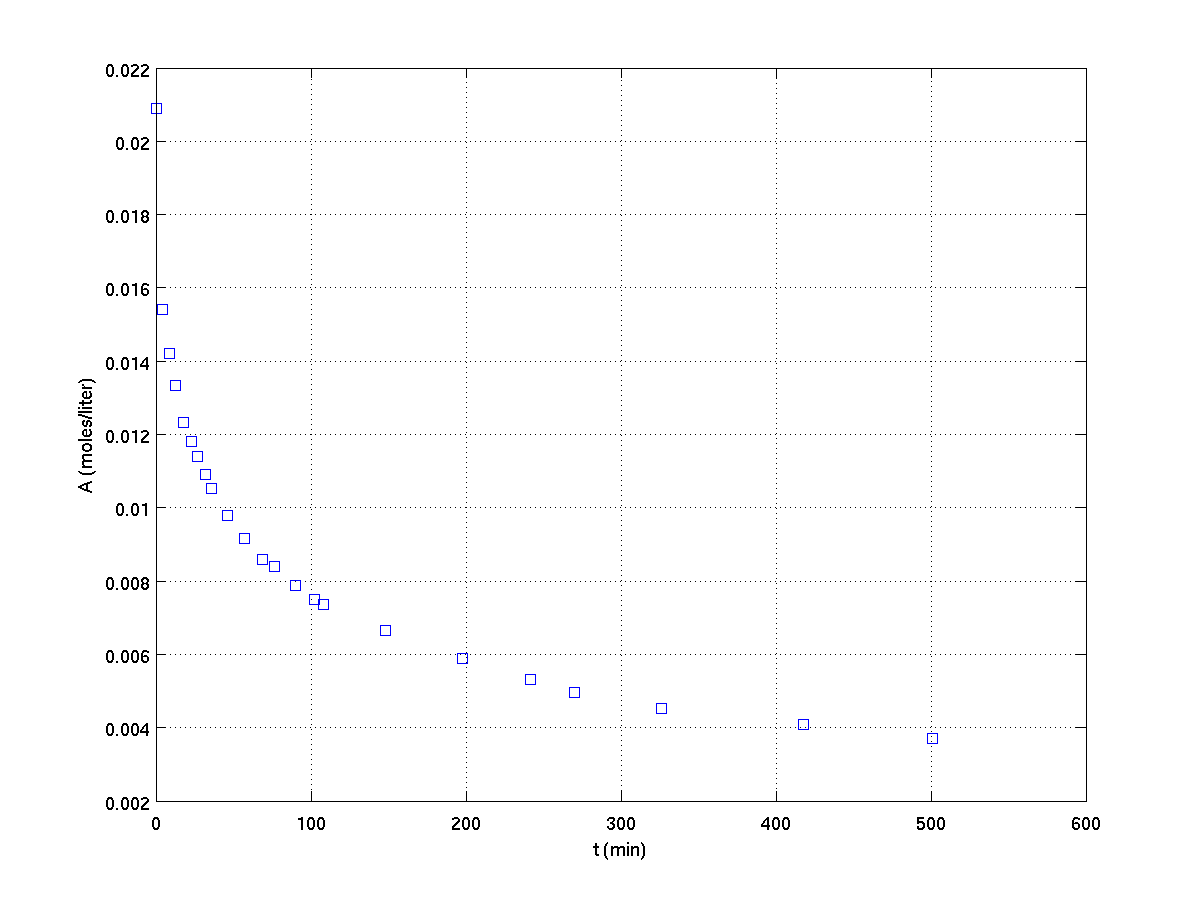
\includegraphics[scale=1.00,clip=true,viewport=0.5in 0.2in 11.5in 8.5in]{himmelAobs.eps}
\end{center}
\caption{Chemical reactions example (Section \ref{sc-gmc-dram-chem-ex}):
plot of concentrations $A$ observed at 23 different instants.
The information for this plot comes from Table \ref{tab-dram-chem-ex-sys-y1-obs}.
}
\label{fig-dram-chem-ex-sys-y1-obs}
\end{figure}

\clearpage
\subsection{Obtaining Posterior Distributions}

Given all this information, we compute the posterior distributions of $k_1$, $k_2$ and $k_3$ with algorithms MH, DR, AM and DRAM using the options presented in
Table \ref{tab-dram-chem-ex-alg-params}.

\begin{table}[h!]
\begin{center}
\begin{tabular}{|c|c|c|c|c|}
\hline
Option                                            & \multicolumn{4}{c|}{Value}                                   \\
\hline
\hline
$n_{\text{sip}}$                                  & \multicolumn{4}{c|}{$3$}                                     \\
\hline
$n_{\text{soq}}$                                  & \multicolumn{4}{c|}{$1$}                                     \\
\hline
$n_{\text{chain}}$                                & \multicolumn{4}{c|}{$1001,~5001$}                            \\
\hline
\hline
$V_{\text{prior}}[\ell_j(\cdot)]$,
$1\leqslant j\leqslant n_{\text{soq}}$            & \multicolumn{4}{c|}{$2.1876e-08$}                            \\
\hline
Update $V^{(k)}[\ell_j(\cdot)]$ for $k>0$?        & \multicolumn{4}{c|}{Yes}                                     \\
\hline
${\tilde{n}}_j$'s                                 & \multicolumn{4}{c|}{23}                                      \\
\hline
$a_j$'s                                           & \multicolumn{4}{c|}{1.}                                      \\
\hline
\hline
$-$                                               & ~~MH~~            & ~~DR~~       & ~~AM~~       & DRAM       \\
\hline
$n_e$                                             &                   &              &              &            \\
\hline
$\gamma_l$,
$1\leqslant l\leqslant n_e$                       &                   &              &              &            \\
\hline
\hline
$t_0$                                             &                   &              &              &            \\
\hline
$p_0$                                             &                   &              &              &            \\
\hline
$\eta$                                            &                   &              &              &            \\
\hline
$\epsilon$                                        &                   &              &              &            \\
\hline
\end{tabular}
\caption{Chemical reactions example (Section \ref{sc-gmc-dram-chem-ex}):
algorithm parameters used.
}
\label{tab-dram-chem-ex-alg-params}
\end{center}
\end{table}

For each of the four algorithms in Table \ref{tab-dram-chem-ex-alg-params}
we compute two chains: the first with $1,001$ positions and the second with $5,001$ positions.
The first position of the first chain is the initial position given in Table \ref{tab-dram-chem-ex-sys-input-params}, while
the second position of the second chain is the final position computed in the first chain.
Tables \ref{tab-dram-chem-ex-results-1} and \ref{tab-dram-chem-ex-results-2} present the results for all combinations of four
algorithms and two chains.

\begin{table}[h!]
\begin{center}
\begin{tabular}{|c|c|c|c|c|c|c|c|c|}
\hline
Method & Run      & $\text{rej}$           & $\text{oor}$           & $i$ & $\langle\theta_i\rangle$ & $\sigma_{\text{bm}}(\theta_i)$ & $\text{gew}(\theta_i)$ & $\tau_{\text{int}}(\theta_i)$ \\
       & Time (s) &                        &                        &     &                          &                                &                        &                               \\
\hline
\hline
       &          &                        &                        & $1$ &                          &                                &                        &                               \\
\cline{5-9}
MH     &          &                        &                        & $2$ &                          &                                &                        &                               \\
\cline{5-9}
       &          &                        &                        & $3$ &                          &                                &                        &                               \\
\hline
\hline
       &          &                        &                        & $1$ &                          &                                &                        &                               \\
\cline{5-9}
DR     &          &                        &                        & $2$ &                          &                                &                        &                               \\
\cline{5-9}
       &          &                        &                        & $3$ &                          &                                &                        &                               \\
\hline
\hline
       &          &                        &                        & $1$ &                          &                                &                        &                               \\
\cline{5-9}
AM     &          &                        &                        & $2$ &                          &                                &                        &                               \\
\cline{5-9}
       &          &                        &                        & $3$ &                          &                                &                        &                               \\
\hline
\hline
       &          &                        &                        & $1$ &                          &                                &                        &                               \\
\cline{5-9}
DRAM   &          &                        &                        & $2$ &                          &                                &                        &                               \\
\cline{5-9}
       &          &                        &                        & $3$ &                          &                                &                        &                               \\
\hline
\end{tabular}
\caption{Chemical reactions example (Section \ref{sc-gmc-dram-chem-ex}):
results from the first chain, with $n_{\text{chain}}=1001$ samples,
for each of the $n_{\text{sip}}=4$ parameters $\theta_i$, $1\leqslant i\leqslant n_{\text{sip}}$.
}
\label{tab-dram-chem-ex-results-1}
\end{center}
\end{table}

\begin{table}[h!]
\begin{center}
\begin{tabular}{|c|c|c|c|c|c|c|c|c|}
\hline
Method & Run      & $\text{rej}$           & $\text{oor}$           & $i$ & $\langle\theta_i\rangle$ & $\sigma_{\text{bm}}(\theta_i)$ & $\text{gew}(\theta_i)$ & $\tau_{\text{int}}(\theta_i)$ \\
       & Time (s) &                        &                        &     &                          &                                &                        &                               \\
\hline
\hline
       &          &                        &                        & $1$ &                          &                                &                        &                               \\
\cline{5-9}
MH     &          &                        &                        & $2$ &                          &                                &                        &                               \\
\cline{5-9}
       &          &                        &                        & $3$ &                          &                                &                        &                               \\
\hline
\hline
       &          &                        &                        & $1$ &                          &                                &                        &                               \\
\cline{5-9}
DR     &          &                        &                        & $2$ &                          &                                &                        &                               \\
\cline{5-9}
       &          &                        &                        & $3$ &                          &                                &                        &                               \\
\hline
\hline
       &          &                        &                        & $1$ &                          &                                &                        &                               \\
\cline{5-9}
AM     &          &                        &                        & $2$ &                          &                                &                        &                               \\
\cline{5-9}
       &          &                        &                        & $3$ &                          &                                &                        &                               \\
\hline
\hline
       &          &                        &                        & $1$ &                          &                                &                        &                               \\
\cline{5-9}
DRAM   &          &                        &                        & $2$ &                          &                                &                        &                               \\
\cline{5-9}
       &          &                        &                        & $3$ &                          &                                &                        &                               \\
\hline
\end{tabular}
\caption{Chemical reactions example (Section \ref{sc-gmc-dram-chem-ex}):
results from the second chain, with $n_{\text{chain}}=5001$ samples,
for each of the $n_{\text{sip}}=4$ parameters $\theta_i$, $1\leqslant i\leqslant n_{\text{sip}}$.
}
\label{tab-dram-chem-ex-results-2}
\end{center}
\end{table}

\clearpage
\subsection{A Simple Prediction}

See Figure \ref{fig-dram-chem-ex-prediction}.

\begin{figure}[h!]
\begin{center}
%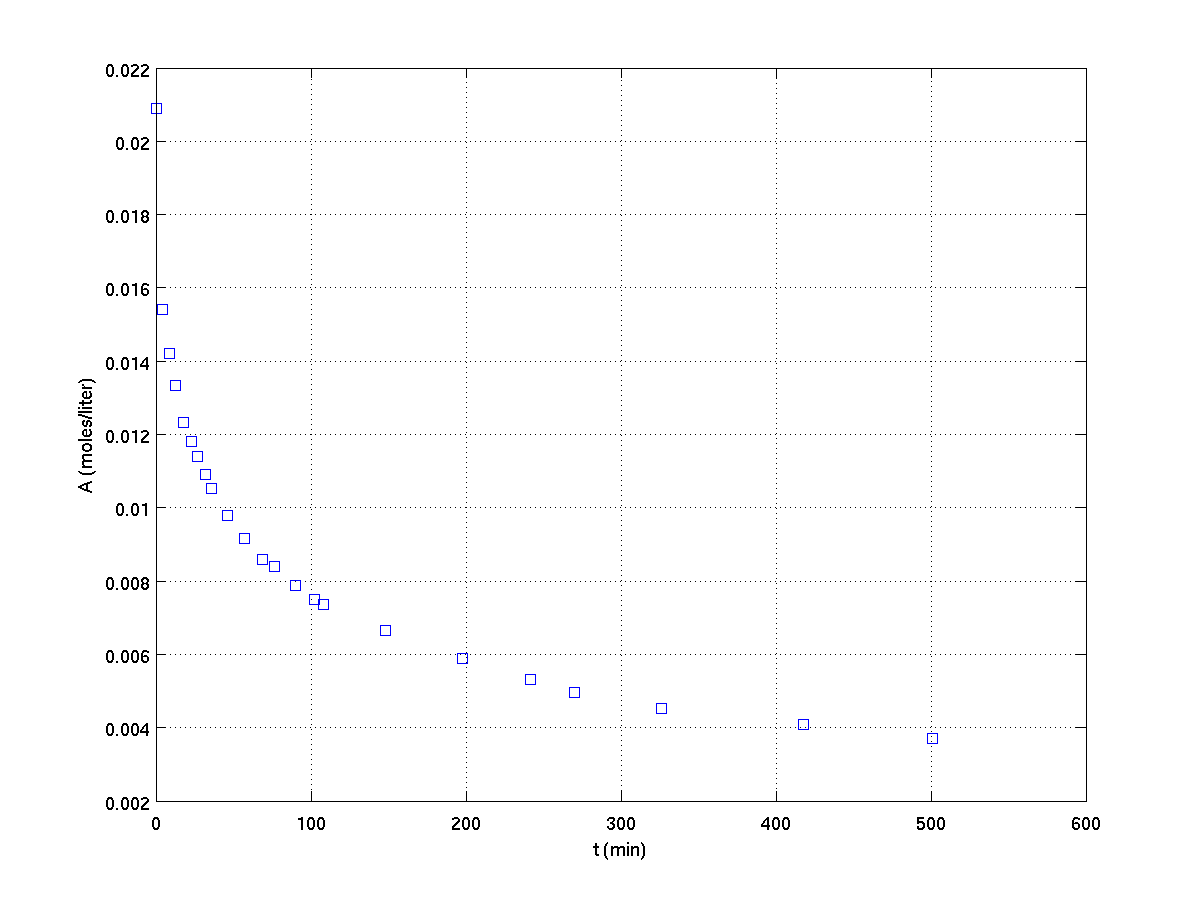
\includegraphics[scale=1.00,clip=true,viewport=0.5in 0.2in 11.5in 8.5in]{himmelAobs.eps}
\end{center}
\caption{Chemical reactions example (Section \ref{sc-gmc-dram-chem-ex}):
prediction of all concentrations, obtained with the mean of the chain of 5001 positions obtained with DRAM.
}
\label{fig-dram-chem-ex-prediction}
\end{figure}

\clearpage
\subsection{Comparison With the MCMC Matlab Toolbox}

See Table \ref{tab-dram-chem-ex-comparison}.

\begin{table}[h!]
\begin{center}
\begin{tabular}{|c|c|c|c|c|c|c|c|c|c|c|c|}
\hline
Method & \multicolumn{2}{c|}{Run Time (s)} & \multicolumn{2}{c|}{$\text{rej}$} & $i$ & \multicolumn{2}{c|}{$\langle\theta_i\rangle$} & \multicolumn{2}{c|}{$\text{gew}(\theta_i)$} & \multicolumn{2}{c|}{$\tau_{\text{int}}(\theta_i)$} \\
\cline{2-5}\cline{7-12}
       & Kit            & Box              & Kit           & Box               &     & Kit                  & Box                    & Kit                 & Box                   & Kit                     & Box                      \\
\hline
\hline
       &                &                  &               &                   & $1$ &                      &                        &                     &                       &                         &                          \\
\cline{6-12}
MH     &                &                  &               &                   & $2$ &                      &                        &                     &                       &                         &                          \\
\cline{6-12}
       &                &                  &               &                   & $3$ &                      &                        &                     &                       &                         &                          \\
\hline
       &                &                  &               &                   & $1$ &                      &                        &                     &                       &                         &                          \\
\cline{6-12}
DR     &                &                  &               &                   & $2$ &                      &                        &                     &                       &                         &                          \\
\cline{6-12}
       &                &                  &               &                   & $3$ &                      &                        &                     &                       &                         &                          \\
\hline
       &                &                  &               &                   & $1$ &                      &                        &                     &                       &                         &                          \\
\cline{6-12}
AM     &                &                  &               &                   & $2$ &                      &                        &                     &                       &                         &                          \\
\cline{6-12}
       &                &                  &               &                   & $3$ &                      &                        &                     &                       &                         &                          \\
\hline
       &                &                  &               &                   & $1$ &                      &                        &                     &                       &                         &                          \\
\cline{6-12}
DRAM   &                &                  &               &                   & $2$ &                      &                        &                     &                       &                         &                          \\
\cline{6-12}
       &                &                  &               &                   & $3$ &                      &                        &                     &                       &                         &                          \\
\hline
\end{tabular}
\caption{Chemical reactions example (Section \ref{sc-gmc-dram-chem-ex}):
comparison between the PECOS Toolkit (``kit'') and the MCMC Matlab Toolbox (``box'', \cite{mcmctool}), w.r.t. to the first chain of 1001 positions generated by each method.
}
\label{tab-dram-chem-ex-comparison}
\end{center}
\end{table}

See Figures
\ref{fig-dram-chem-ex-comparison-MH-theta1-chain1},
\ref{fig-dram-chem-ex-comparison-DR-theta1-chain1},
\ref{fig-dram-chem-ex-comparison-AM-theta1-chain1} and
\ref{fig-dram-chem-ex-comparison-DRAM-theta1-chain1}.

\begin{figure}[h!]
\begin{center}
%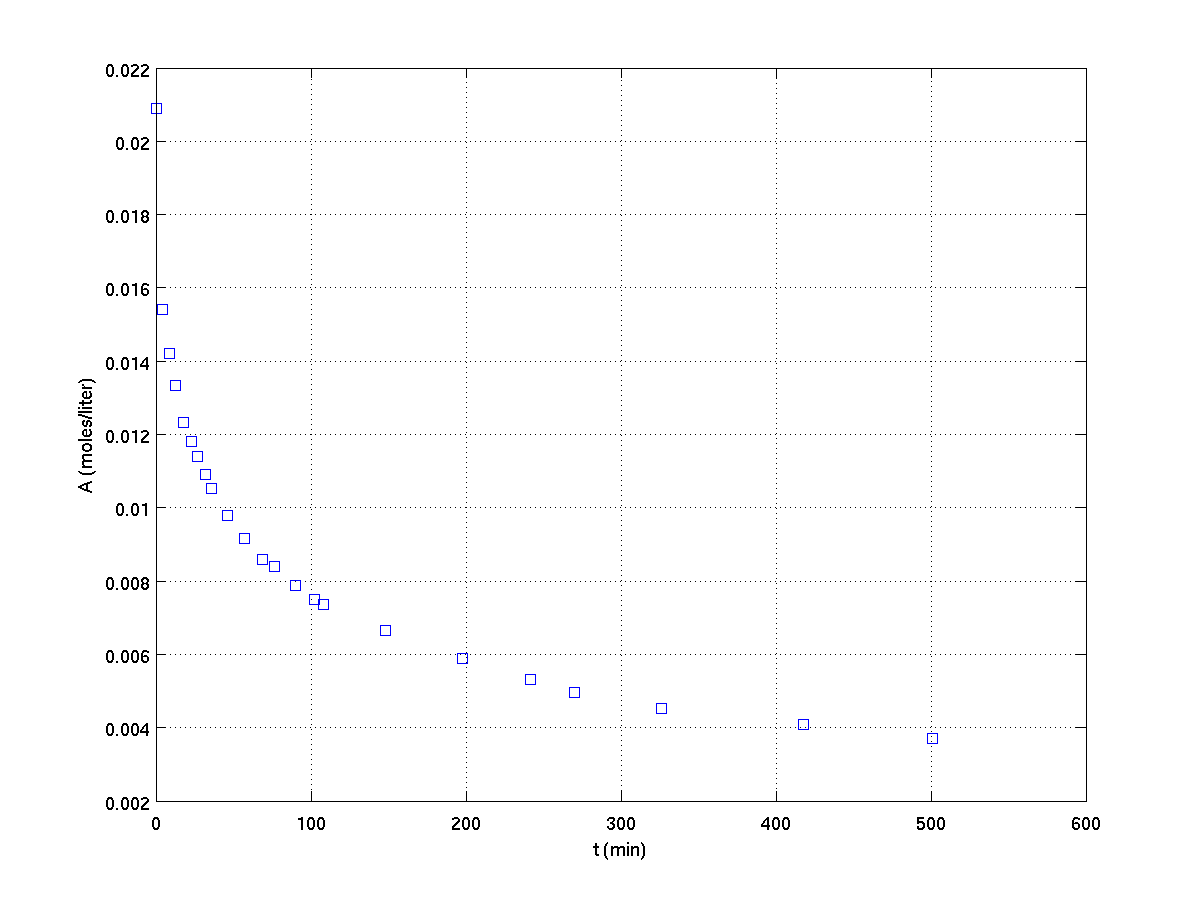
\includegraphics[scale=1.00,clip=true,viewport=0.5in 0.2in 11.5in 8.5in]{himmelAobs.eps}
\end{center}
\caption{Chemical reactions example (Section \ref{sc-gmc-dram-chem-ex}):
visual comparison between the MH algorithm results from the PECOS Toolkit (``kit'') and the MCMC Matlab Toolbox (``box'', \cite{mcmctool}), w.r.t. to the 1001 values of $\theta_1$ from the first chain generated by MH.
}
\label{fig-dram-chem-ex-comparison-MH-theta1-chain1}
\end{figure}

\begin{figure}[h!]
\begin{center}
%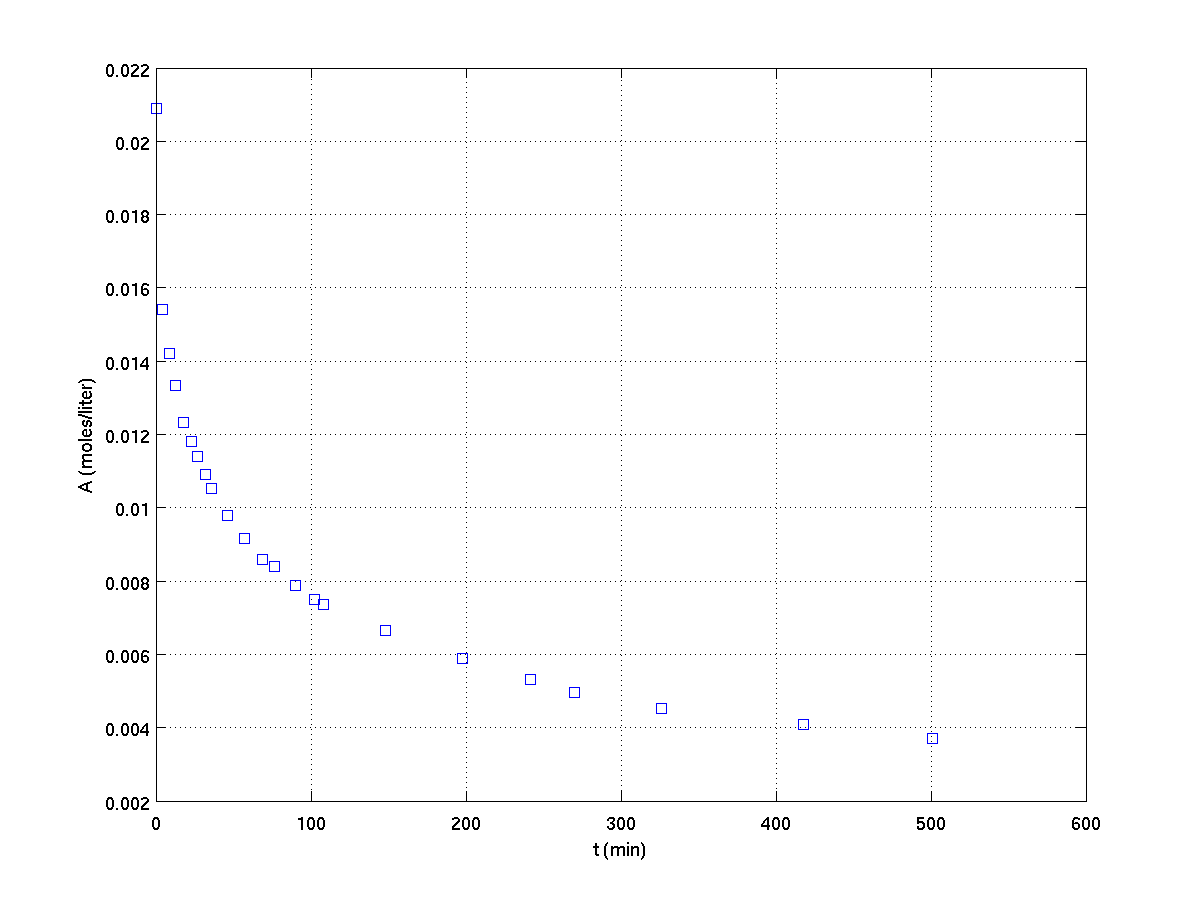
\includegraphics[scale=1.00,clip=true,viewport=0.5in 0.2in 11.5in 8.5in]{himmelAobs.eps}
\end{center}
\caption{Chemical reactions example (Section \ref{sc-gmc-dram-chem-ex}):
visual comparison between the DR algorithm results from the PECOS Toolkit (``kit'') and the MCMC Matlab Toolbox (``box'', \cite{mcmctool}), w.r.t. to the 1001 values of $\theta_1$ from the first chain generated by DR.
}
\label{fig-dram-chem-ex-comparison-DR-theta1-chain1}
\end{figure}

\begin{figure}[h!]
\begin{center}
%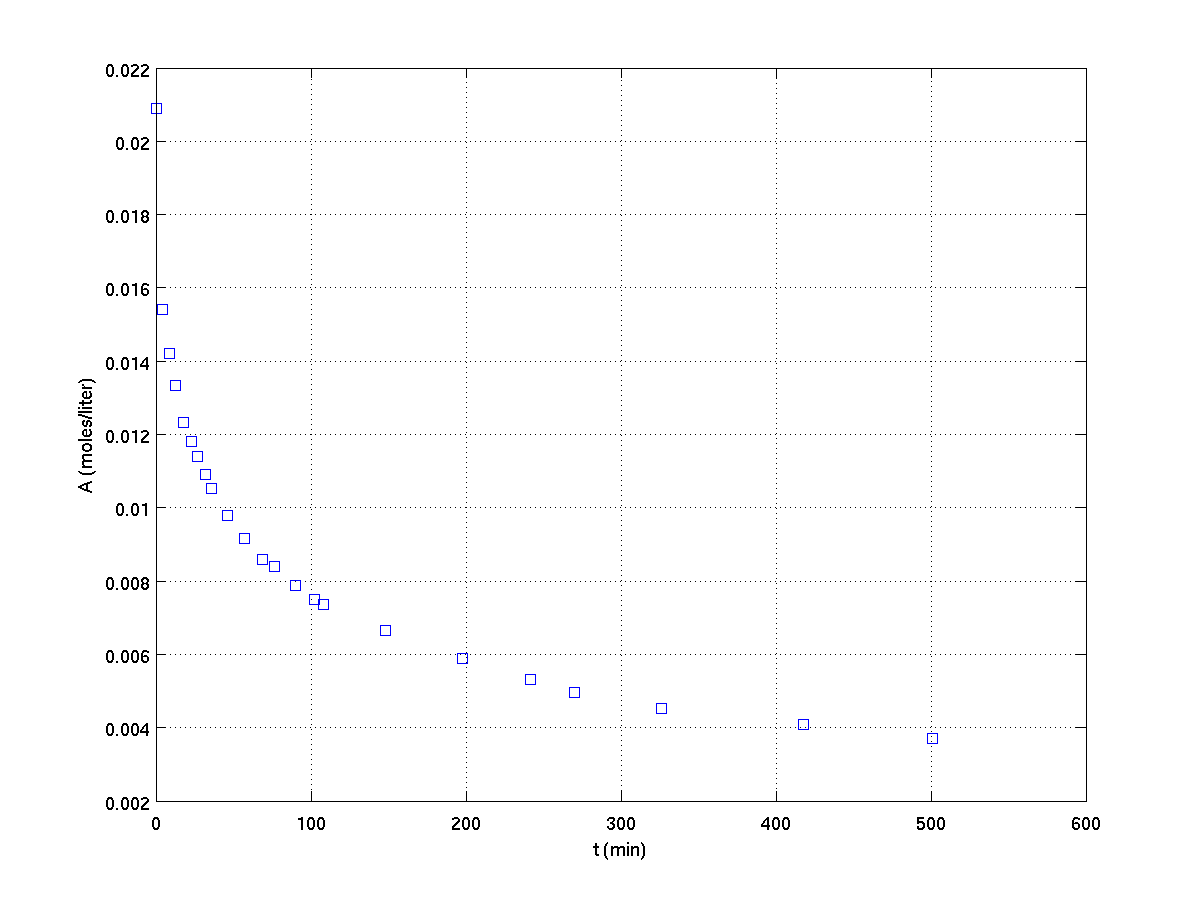
\includegraphics[scale=1.00,clip=true,viewport=0.5in 0.2in 11.5in 8.5in]{himmelAobs.eps}
\end{center}
\caption{Chemical reactions example (Section \ref{sc-gmc-dram-chem-ex}):
visual comparison between the AM algorithm results from the PECOS Toolkit (``kit'') and the MCMC Matlab Toolbox (``box'', \cite{mcmctool}), w.r.t. to the 1001 values of $\theta_1$ from the first chain generated by AM.
}
\label{fig-dram-chem-ex-comparison-AM-theta1-chain1}
\end{figure}

\begin{figure}[h!]
\begin{center}
%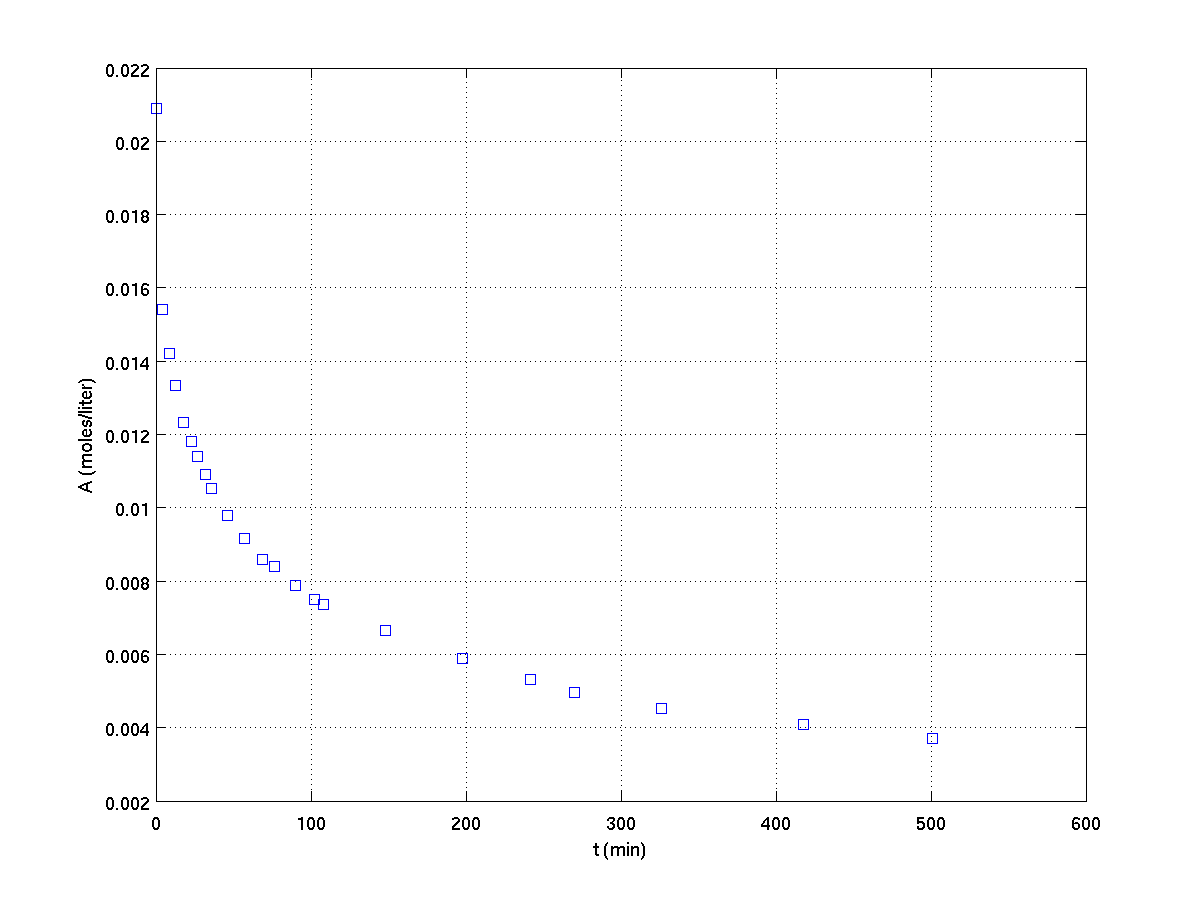
\includegraphics[scale=1.00,clip=true,viewport=0.5in 0.2in 11.5in 8.5in]{himmelAobs.eps}
\end{center}
\caption{Chemical reactions example (Section \ref{sc-gmc-dram-chem-ex}):
visual comparison between the DRAM algorithm results from the PECOS Toolkit (``kit'') and the MCMC Matlab Toolbox (``box'', \cite{mcmctool}), w.r.t. to the 1001 values of $\theta_1$ from the first chain generated by DRAM.
}
\label{fig-dram-chem-ex-comparison-DRAM-theta1-chain1}
\end{figure}

\clearpage

\section{Example With Algae Populations}\label{sc-gmc-dram-algae-ex}

\subsection{Problem Statement}
$~$\\

\subsection{Obtaining Posterior Distributions}
$~$\\

\subsection{Predictions}
$~$\\

\clearpage

\section{Planned Features for Next Releases}\label{sc-gmc-planned-features}
With respect to Markov Chain Monte Carlo methods, the following features are planned for the next versions of the PECOS Toolkit for Predictive Engineering:
\begin{enumerate}
\item remove dependencies on the MCMC Toolbox w.r.t. displaying output data,
\item compute predictions for the algae example,
\item chain convergence tests,
\item regression tests,
\item capability of running over parallel environments using Trilinos,
\item integration with the DAKOTA Toolkit,
\item support different types of output formats, not only MATLAB,
\item hyperprior models,
\item algorithms for multimodal distributions,
\item Gibbs sampler,
\item capability of running over parallel environments using PETSc.
\end{enumerate}
 
